% Created 2020-07-09 Thu 19:42
% Intended LaTeX compiler: pdflatex
\documentclass[a4paper]{apa6}
\usepackage[utf8]{inputenc}
\usepackage[T1]{fontenc}
\usepackage{graphicx}
\usepackage{grffile}
\usepackage{longtable}
\usepackage{wrapfig}
\usepackage{rotating}
\usepackage[normalem]{ulem}
\usepackage{amsmath}
\usepackage{textcomp}
\usepackage{amssymb}
\usepackage{capt-of}
\usepackage{hyperref}
\affiliation{King's College London}
\shorttitle{Multi-scale modelling of carbon migration in iron}
\usepackage{breakcites}
\usepackage{apacite}
\usepackage{paralist}
\let\itemize\compactitem
\let\description\compactdesc
\let\enumerate\compactenum
\author{Tigany Zarrouk}
\date{\today}
\title{Multi-scale investigation of dislocation mediated carbon migration in iron}
\hypersetup{
 pdfauthor={Tigany Zarrouk},
 pdftitle={Multi-scale investigation of dislocation mediated carbon migration in iron},
 pdfkeywords={},
 pdfsubject={},
 pdfcreator={Emacs 26.3 (Org mode 9.1.9)}, 
 pdflang={English}}
\begin{document}

\maketitle
\tableofcontents

\begin{abstract}

*Abstract*

We investigate the validity of a dislocation-assisted carbon migration
mechanism underpinning the formation of dark etching regions in
bearing steels undergoing high-cycle fatigue through use of a
multi-scale approach: from quantum mechanics,
to stochastic simulations. We start from tight binding simulations of
$1/3\langle 111 \rangle$ screw dislocations to obtain the 2-d Peierls
potential and Fe-C binding energies. These become ingredients for a line-tension
model of the $1/3\langle 111 \rangle$ screw dislocation to obtain the kink-pair formation
energy as a function of stress and carbon concentration. Finally,
3-d kinetic Monte-Carlo simulations of dislocations in an environment
of carbon are used to ascertain which temperature and stress regimes
dislocation-assisted carbon migration is a valid mechanism. 

\end{abstract}


\section{Introduction}
\label{sec:orge83a9bb}

\section{Computational Method}
\label{sec:org811f961}

\begin{itemize}
\item Use tight-binding model of Paxton and Elsaetter \cite{Paxton2013}.
\item Generate dislocations using anisotropic elasticity theory.
\item Create clusters of dislocations in both easy and hard core
configurations.
\item Place carbon in octahedral sites around the core
\item Calculate corrections (ZPE etc)
\end{itemize}


\section{Results}
\label{sec:orgc4b8119}



\subsection{Peierls Potential}
\label{sec:orge77bc3e}

To determine the Peierls potential, we followed the procedure detailed in Itakura
\cite{Itakura2012}. Quadrupolar arrays of dislocations were constructed by placing dislocations of
antiparallel \(1/2\langle 111\rangle\) Burgers vectors in an "S" arrangement \cite{Clouet2012}, with
initial displacements determined by the anisotropic elasticity solutions. These displacements
were modified to be periodic, thereby removing artificial stacking faults which would appear
between periodic images after the introduction of the dipole. This was achieved by the subraction
of a linear error term from the superposition of displacement fields arising from the
dislocations in the simulation cell and its periodic images \cite{vasilybulatov2006}. To accomodate
for the internal stress upon introduction of the dislocation dipole into a simulation cell, an
elastic strain was imposed on the cell, resulting in an extra tilt component being added to the
cell vectors \cite{Clouet2012,vasilybulatov2006}. Simulation cells were constructed with different
initial core positions, which were sampled from the triangular region "EHS" (easy, hard and
split) core positions, as detailed in \ref{fig:peierlspot}. To fix the dislocation positions during
relaxation, the three atoms surrounding the easy core, for each dislocation, were fixed during
relaxation.


        \begin{table}
    \begin{tabular}{c}
	     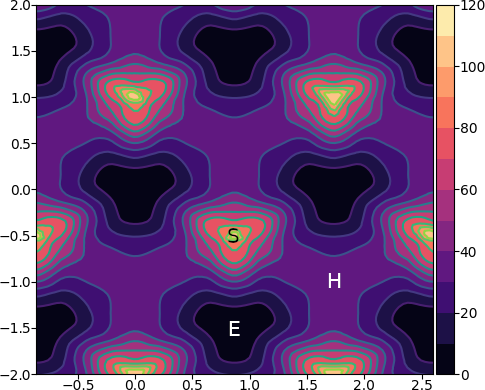
\includegraphics[width=0.4\textwidth]{../Images/itakura_dislocation_energy_landscape_2_labelled.png} \\
             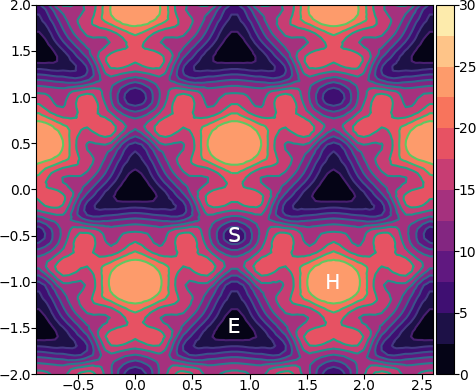
\includegraphics[width=0.4\textwidth]{../Images/tbe_dislocation_energy_landscape_pure_labelled.png}  \\
    \end{tabular}		
\caption{Comparison of 2d Peierls potentials of the $1/2\langle 111\rangle$ screw dislocation between DFT cite:Itakura2012 (top) and tight-binding (bottom). Data was interpolated using cubic splines. Energies are in $meV$, with x and y scales in units of $\sqrt{2} a_{\text{bcc}} = 2\sqrt{2/3}b$. "E", "H" and "S" correspond to easy, hard and split core positions respectively, with the latter also corresponting to atomic positions. The relative energies between the different core positions is smaller in tight-binding compared to DFT. The split core as seen in tight-binding is reminiscent of EAM potentials, where the split core energy is lower than that of the hard core. Some of this discrepancy can be attributed to the difference in simulation method: the cluster method may inhibit the relaxation of the core more than quadrupolar cells, due to finite size effects.}
	\label{fig:peierlspot}
    \end{table}

Comparison of 2d Peierls potentials of the \(1/2\langle 111\rangle\) screw dislocation between
DFT can by found in \cite{Itakura2012}. Data was interpolated using 2d cubic splines. "E", "H"
and "S" correspond to easy, hard and split core positions respectively, with the latter also
corresponding to atomic positions. The relative energies between the different core
positions is smaller in tight-binding compared to DFT; most notably, the energies. This is
an artifact in the model, which has been validated in NEB calculations of the \(1/2\langle
	111\rangle\) screw dislocation Peierls barrier, as calculated with NEB, is roughly half that
when compared to DFT \textbf{INSERT LUKES THESIS REFERENCE}. The split core as seen in
tight-binding is reminiscent of EAM potentials, where the split core energy is lower than
that of the hard core.

This may be attributed to lack of core electron	repulsion, resulting from the sd-iron tight-binding model. 

\subsection{Hard and easy core relaxations}
\label{sec:orgd64a5d5}

To determine the binding energy of carbon to dislocations, we used the
cluster method; where the simulation cells consist of a circular cluster of
atoms, split into two regions, with a single dislocation introduced into the
centre by using the anisotropic elasticity solutions. Each of the clusters
were centred on the easy or hard core positions. The cluster of atoms was
split into two regions: a central region of dynamic atoms with radius \(R_1\),
and an annulus of atoms, between \(R_1\) and \(R_2\), which were fixed to the anisotropic
elasticity solutions. 

Initially, large cells of with \(R_1 = 6\sqrt{2}a_{\text{bcc}}\), and \(R_2 =
   7\sqrt{2}a_{\text{bcc}}\) and depth of single burger's vector, were relaxed
for both the easy and hard cores, which consisted of 522 and 540 atoms
respectively. The three atoms surrounding the core were constrained, to only
relax in \(X-Y\) plane, to stop the core from moving upon relaxation. The
k-point sampling mesh for each of these cells was 1x1x24, with a charge
tolerance for self-consistency of \(1e-6\). Atoms were relaxed until the force
on each atom was less than \(1e-3\) eV/\AA{}.  

From the relaxed cells, a smaller region of 174 atoms, with \(R_1 =
   3\sqrt{2}a_{\text{bcc}}\), and \(R_2 = 4\sqrt{2}a_{\text{bcc}}\), was cut from
the dynamic regions. This smaller cell was extended to a thickness of 3b in
the Z direction. Carbon interstitials were inserted into octahedral sites
near the dislocation core, in the middle layer. Exploiting reflection and
rotational symmetry allowed us to use only 10 interstitial
sites to obtain the binding energies of carbon \$\(\sim\) 1.8\$b from the core. 


As found in DFT simulations by Ventelon \cite{Ventelon2015}, when a carbon was placed in the
vicinity of a relaxed easy dislocation core---in either of the two nearest, distinguishable,
octahedral sites---a spontaneous reconstruction of the dislocation core occurred: from easy to
hard. Upon reconstruction, the dislocation core moved to a neighbouring triangle, when looking along the \(\langle
   111\rangle\) direction, where the carbon found itself situated in the centre.


Plot of dislocation energy as function of cluster size. 
\begin{center}
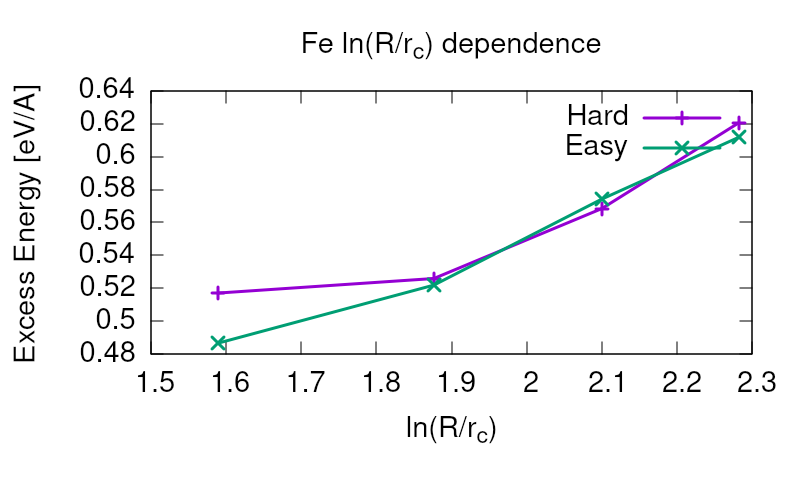
\includegraphics[width=.9\linewidth]{/home/tigany/Documents/docs/Management/Images/img_fe_size_dependence_on_log_of_core_radius.png}
\end{center}



\begin{table}	
    \begin{tabular}{c}
 	          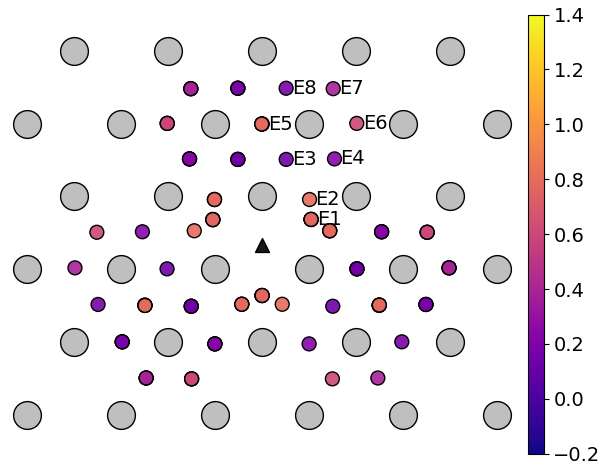
\includegraphics[width=0.45\textwidth]{../Images/easy_core_fe_C_positioning_energies.png}  \\
 	          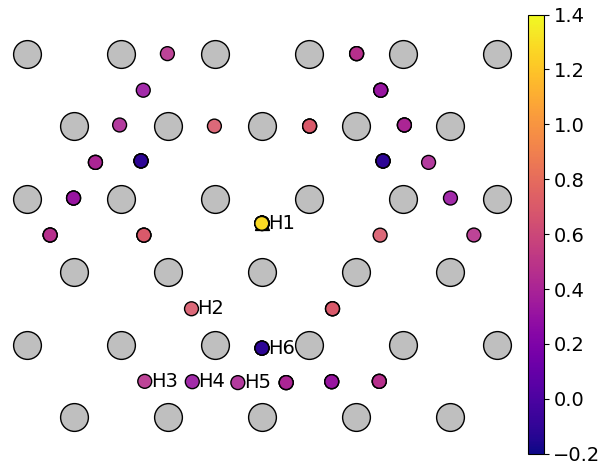
\includegraphics[width=0.45\textwidth]{../Images/hard_core_fe_C_positioning_energies.png}  \\

     	     \end{tabular}		
\caption{ Final positions and binding energies (eV) of carbon around the easy core (top) and hard core (bottom). The core was constrained by fixing the top and bottom three atoms surrounding each of the cores. As shown by Ventelon cite:Ventelon2015, the first and second closest octahedral sites to the hard core have their minimum energy inside the hard core. }
   \end{table}


Following the paper by Itakura
\cite{itakura13_effec_hydrog_atoms_screw_disloc} we calculated the
binding energy of carbon each of the screw dislocation cores. 

The solution energy is given by 
\[ E_s = E_{\text{d + C}} - E_{\text{d}} - E_{\text{C oct.}}, \]
where \(E_{\text{d + C}}\) is the total energy of a relaxed cluster with a
carbon interstitial and a dislocation, \(E_{\text{d}}\) is the total
energy of a relaxed cluster with a dislocation and \(E_{\text{C
    oct.}}\) is the total energy of relaxed a cluster with a single carbon in
an octahedral site.

The zero-point energy is calculated as in Itakura. A 3x3 Hessian
matrix is constructed by taking the numerical derivative of the
forces observed on the carbon atom after displacement by \(\pm 0.015 \AA\) in each of the \(X\), \(Y\) and \(Z\)
directions. The zero-point energy is given by

\[ E_z = \frac{1}{2} \sum_{i=1}^3 \frac{h}{2\pi} \sqrt{ k_i /
    m_{\text{C}} },  \]
where \(k_i\) are the eigenvalues of the Hessian and \(m_\text{C}\) is
the mass of carbon. 

    The ZPE corrected solution energy is given by 
    \[ E^{\text{Z}}_{s} = E_s + E_z - E_{z\text{C oct.}},  \]
v
    where \(E_{z\text{C oct.}} = 202.5 meV\) is the zero-point energy of carbon
    situated in an octahedral site in a perfect cluster of the same size. 

Table of relaxed 


\begin{center}
\begin{tabular}{lrrr}
Site Type & \(E_b^{z}\) eV & distance from core [b] & distance from core \AA{}\\
\hline
E1 & 0.775 & 0.57 & 1.413699\\
E2 & 0.793 & 0.70 & 1.732527\\
E3 & 0.139 & 0.99 & 2.458179\\
E4 & 0.234 & 1.21 & 3.001665\\
E5 & 0.791 & 1.36 & 3.369997\\
E6 & 0.603 & 1.66 & 4.129084\\
E7 & 0.388 & 1.89 & 4.703422\\
E8 & 0.178 & 1.77 & 4.409563\\
H1/H2 & 1.291 & 0.00 & 0.006472\\
H3/H4 & 0.698 & 1.19 & 2.960187\\
H5 & 0.467 & 2.12 & 5.287079\\
H6 & 0.316 & 1.91 & 4.746490\\
H7 & 0.409 & 1.80 & 4.483550\\
H8 & -0.114 & 1.40 & 3.480325\\
\end{tabular}
\end{center}


These binding energies agree well with experiment and previous calculations. The maximum binding energy found by 


Distance dependence of binding energies. 

\begin{center}
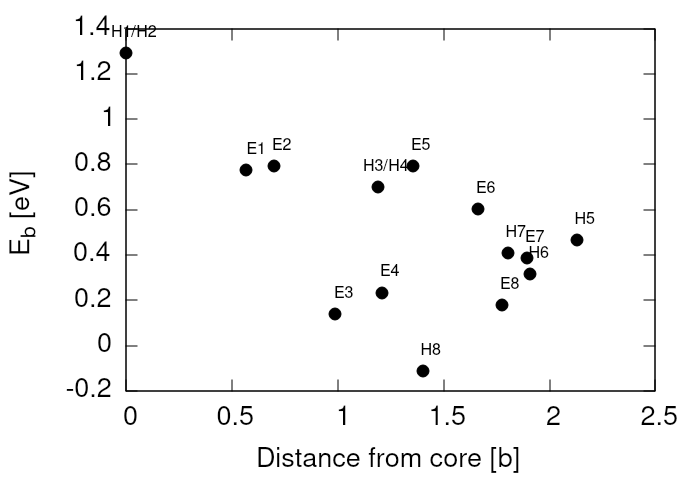
\includegraphics[width=.9\linewidth]{/home/tigany/Documents/docs/Management/Images/temp_binding_energy_distance_C_Fe.png}
\end{center}



\section{Bibliography}
\label{sec:orgf202318}
\label{org40ca11c}

\bibliographystyle{unsrt}
\bibliography{../bibliography/org-refs}
\end{document}